\section{ACL en use}

Dans cette session on verrais les uses des ACL dans les système d'aujourd'hui. 

\subsection{ACL Kernel Patches}
Les ACL \emph{patches} ont été ajouter dans le noyaux Linux depuis November 2002. Cette \emph{patches} implémentent le POSIX 1003.1e brouillon 17 et elles ont été ajoute dans le version 2.5.46 du noyaux. Donc le support ACL et aussi présent dans le dernière version du noyaux aujourd'hui. Depuis 2004 le support aux ACL étions disponible pour les système de fichier Ext2, Ext3, IBM JFS, ReiserFS et SGI XFS. Les ACL sont supporte aussi pour le système NFS, par contre, il y a quelques problèmes de sécurité connu\cite{nfs_problem}. 

Aujourd'hui c'est assez simple pour ajouter le supporte aux ACL dans les distribution Linux comme Ubuntu ou Debian. On verrais les pas pour ajouter ce supporte après.

\subsection{Mac OSX}
Le système de exploitation Mac OSX (10.6.2 Snow Leopard dans le moment de écriture de ce article) a aussi les supporte aux ACL complètement intégrée dans l'interface de utilisateur (\ref{fig:img_mac-acl}). 

\begin{figure}[htbp]
	\centering
		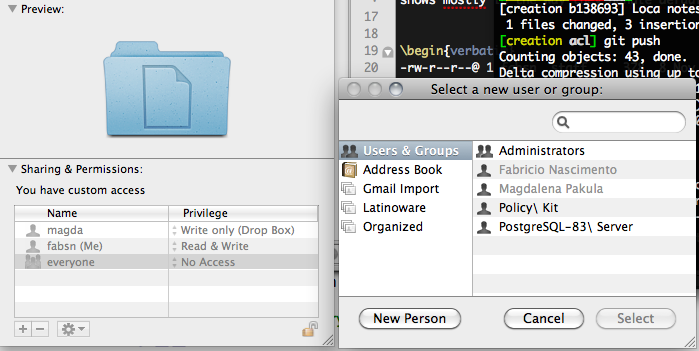
\includegraphics[height=3in]{img/mac-acl.png}
	\caption{Mac OSX Snow Leopard ACL Interface}
	\label{fig:img_mac-acl}
\end{figure}


%Parler un peut plus de Mac.


\subsection*{Using ACL in Linux}


%References 
Les dernière version des distribution Debian ou Ubuntu, comme Ubuntu 9.10, dèjá vient avec le supporte aux ACL. Dans le Ubuntu 8.10 l'application Nautilus, qui est responsable pour la visualisation du système de fichier, contenait une interface pour les ACL, apparentement l'interface a été discontinue et le Nautilus du Ubuntu 9.10 n'en y a pas encore. Les pas pour ajouter le supporte dans le Ubuntu 9.10 sont:

\begin{verbatim}
1) Installer le paquet des acl. 
user@ubuntu:$ sudo apt-get install acl
 
2) Ajouter le option 'acl' au système de fichier correcte dans le /etc/fstab, comment:
UUID='gros sequence' /dev/hda6 /home ext3 rw,auto,acl 0 1

3) Remounter le systeme de fichier avec le nouvelle option
user@ubuntu:$ sudo mount /home -o remount

\end{verbatim}

\subsection*{Ajouter ACL aux fichiers}

On peut utiliser le commande 'ls -la' pour regarde les permission. Si une fichier contient information de sécurité avancée (comme \emph{access list}) on va voir le "character" '+', comment dans le sortie du command 'ls' ci-dessous (\ref{verb:ls}). Une fichier avec '@' était dire que le fichier a quelque EAs. 

\begin{center}
\label{verb:ls}
\begin{verbatim}
-rw-r--r--@ 1 fabsn  staff     378  8 Nov 15:29 Makefile
-rw-r--r--@ 1 fabsn  staff     618  8 Nov 15:59 README
-rw-r--r--@ 1 fabsn  staff      31  8 Nov 15:15 draft-header
-rw-r--r--@ 1 fabsn  staff      24  8 Nov 15:15 header
drwxr-xr-x@ 2 fabsn  staff     102  8 Nov 15:26 img
-rw-r--r--  1 fabsn  staff     972  8 Nov 15:57 rapport-draft.aux
-rw-r--r--  1 fabsn  staff   18129  8 Nov 15:57 rapport-draft.log
drwxrwxr-x+ 3 fabsn  staff	  1024  8 Nov 20:23 repertoire
\end{verbatim}
\end{center}

Pour voir les ACL on doit utilise le commande \emph{getfacl}. Regarde que les information sont ajoute d'accord avec les définition dans l'introduction sur les ACL dans la tabelle \ref{tab:entree}. 

\begin{verbatim}
fabsn@vadmin:/media/esisar$ getfacl repertoire/
# file: repertoire/
# owner: root
# group: root
user::r-x
user:daemon:rwx
user:bin:rwx
user:fabsn:rwx
user:nobody:rwx
group::r-x
group:admin:rwx
group:fabsn:rwx
mask::rwx
other::r-x	
\end{verbatim}

Aussi on a le commande \emph{setfacl} pour modifier, ou ajouter les permission ACL. Le commande dessous par exemple modifie (-m) les permission du utilisateur \emph{fabsn} pour le répertoire. 

\begin{verbatim}
setfacl -m u:fabsn:r-x repertoire
\end{verbatim}

\subsection*{Exemple}

5	Access ACL Example
Let us start by creating a directory and checking its per- missions. The umask determines which permissions will be masked off when the directory is created. A umask of 027 (octal) disables write access for the owning group and read, write, and execute access for others.
$ umask 027 $ mkdir dir $ ls -dl dir drwxr-x--- ... agruen suse ... dir
The first character ls prints represents the file type (d for directory). The string “rwxr-x---” represents the resulting permissions for the new directory: read, write, and execute access for the owner and read and execute access for the owning group. The dots in the output of ls stand for text that is not relevant here and has been removed.
These base permissions have an equivalent represen- tation as an ACL. ACLs are displayed using the getfacl command.
$ getfacl dir # file: dir # owner: agruen # group: suse user::rwx
group::r-x other::---
The first three lines of output contain the file name, owner, and owning group of the file as comments. Each of the following lines contains an ACL entry for one of the three classes of users: owner, group, and other.
The next example grants read, write, and execute access to user Joe in addition to the existing permis- sions. For that, the -m (modify) argument of setfacl is used. The resulting ACL is again shown using the get- facl command. The –omit-header option to getfacl sup- presses the three-line comment header containing the file name, owner, and owning group to shorten the examples shown.
$ setfacl -m user:joe:rwx dir $ getfacl --omit-header dir user::rwx user:joe:rwx
group::r-x mask::rwx other::---
Two additional entries have been added to the ACL: one is for user Joe and the other is the mask entry. The mask entry is automatically created when needed but not provided. Its permissions are set to the union of the per- missions of all entries that are in the group class, so the mask entry does not mask any permissions.
The mask entry now maps to the group class permis- sions. The output of ls changes as shown next.
$ ls -dl dir drwxrwx---+ ... agruen suse ... dir
An additional “+” character is displayed after the per- missions of all files that have extended ACLs. This seems like an odd change, but in fact POSIX.1 allocates this character position to the optional alternate access method flag, which happens to default to a space charac- ter if no alternate access methods are in use.
The permissions of the group class permissions in- clude write access. Traditionally such file permission bits would indicate write access for the owning group. With ACLs, the effective permissions of the owning group are defined as the intersection of the permissions of the owning group and mask entries. The effective per- missions of the owning group in the example are still r-x, the same permissions as before creating additional ACL entries with setfacl.
The group class permissions can be modified using the setfacl or chmod command. If no mask entry exists, chmod modifies the permissions of the owning group en- try as it does traditionally. The next example removes write access from the group class and checks what hap- pens.


In the following example, we add a default ACL to the directory. Then we check what getfacl shows.
$ setfacl -d -m group:toolies:r-x dir $ getfacl --omit-header dir user::rwx user:joe:rwx
group::r-x mask::rwx other::--- default:user::rwx default:group::r-x default:group:toolies:r-x default:mask::r-x default:other::---
Following the access ACL, the default ACL is printed with each entry prefixed with “default:”. This out- put format is an extension to POSIX.1e that is found on Solaris and Linux. A strict implementation of POSIX 1003.2c would only show the access ACL. The default ACL would be shown with the -d option to getfacl.
We have only specified an ACL entry for the toolies group in the setfacl command. The other entries required for a complete ACL have automatically been copied from the access ACL to the default ACL. This is a Linux- specific extension; on other systems all entries may need to be specified explicitly.
The default ACL contains no entry for Joe, so Joe will not have access (except possibly through group member- ship or the other class permissions).
A subdirectory inherits ACLs as shown next. Unless otherwise specified, the mkdir command uses a value of 0777 as the mode parameter to the mkdir system call, which it uses for creating the new directory. Observe that both the access and the default ACL contain the same entries.
$ mkdir dir/subdir $ getfacl --omit-header dir/subdir user::rwx group::r-x group:toolies:r-x mask::r-x other::--- default:user::rwx default:group::r-x default:group:toolies:r-x default:mask::r-x default:other::---
Files created inside dir inherit their permissions as shown next. The touch command passes a mode value of 0666 to the kernel for creating the file.
All permissions not included in the mode parameter are removed from the corresponding ACL entries. The same has happened in the previous example, but there was no noticeable effect because the value 0777 used for the mode parameter represents a full set of permissions.
Submitted for publication at the USENIX Annual Technical
Conference, San Antonio, Texas, June 2003	5
#effective:r-x
$ touch dir/file $ ls -l dir/file -rw-r-----+ ... agruen suse ... dir/file $ getfacl --omit-header dir/file user::rw- group::r-x group:toolies:r-x mask::r-- other::---
No permissions have been removed from ACL entries in the group class; instead they are merely masked and thus made ineffective. This ensures that traditional tools like compilers will interact well with ACLs. They can create files with restricted permissions and mark the files executable later. The mask mechanism will cause the right users and groups to end up with the expected per- missions.

